\section{Sentiment Analysis Model}
This section outlines the training, testing, and predicting of the BERT model, as well as the dataset chosen for fine-tuning and how it was pre-processed. Most of the functionality shown in this section is contained within the \pinline{BertModel} class under \pinline{toolkit/analysis/model.py}:

\begin{python}
class BertModel(object):
    """
    Class for sentiment analysis using BERT model.
    Attributes:
        tokeniser: BERT tokenizer for tokenizing input text.
        model: BERT model for sentiment classification.
    """
    def __init__(self) -> None:
        self.tokeniser, self.model = None, None
        self.load_model(toolkit.get_dir() + '/models/')
\end{python}

    \subsection{Training}
        This section will outline the steps taken to train and fine-tune the pre-trained BERT model. The majority of the functionality in this section takes place in the \pinline{train()} and \pinline{cross_validate()} methods.

        \subsubsection{Examining the Dataset}
        Before the model can be trained, an appropriate dataset for fine-tuning must be found. As this artefact focuses on social media sentiment analysis, a dataset that has pre-labelled social media posts based on sentiment is needed. For this use-case, the Sentiment140 dataset \citet{sentiment140dataset} was chosen as a widely used and praised dataset for fine-tuning BERT for social media sentiment analysis.

        When calling \pinline{describe()} on the dataset loaded as a Pandas \pinline{DataFrame}, the results are as shown in the table below. This shows that the dataset labels negative sentiment as `0', and positive sentiment as `4', and also appears to have an equal number of negative and positive entries. This quality will be useful as it prevents issues like model generalisation, class imbalance, and overfitting, while allowing for enhanced performance and better feature representation learning.

        \begin{table}[h]
            \centering
            \caption{Dataset description.}
            \label{tbl:datasetdescription}
            \begin{tabular}{c|c|c|c|c|c|c|c|c}
                & Count & Mean & Std & Min & 25\% & 50\% & 75\% & Max \\
                \hline\hline
                Target & 1.60e6 & 2.00 & 2.00 & 0.00 & 0.00 & 2.00 & 4.00 & 4.00 \\
            \end{tabular}
        \end{table}

        We can confirm this by plotting the dataset on a chart using \pinline{pyplot}:

        \begin{figure}[h]
            \centering
            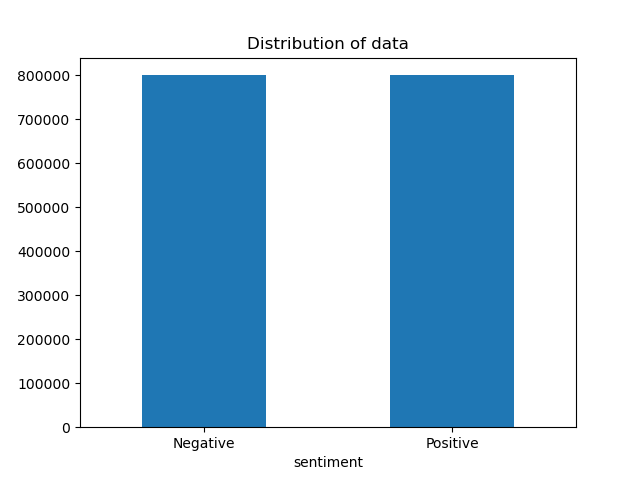
\includegraphics[width=0.6\textwidth]{figures/sentiment140-dataset-distribution.png}
            \caption{Classification distribution in the Sentiment140 dataset.}
        \end{figure}
        \FloatBarrier

        Further examination of the dataset can be accomplished by extracting a positively and negatively classified entry, the dataset provides six features for each post: Target (the sentiment polarity), ID, Date, Flag (the query), User, and Text (the body).

        \FloatBarrier
        \begin{table}[h]
            \centering
            \caption{Example of a positive post.}
            \label{tbl:positive_post}
            \begin{tabular}{p{0.15\linewidth} | p{0.6\linewidth}}
                Attribute & Value \\
                \hline\hline
                Target & 4 \\
                IDs & 1467822272 \\
                Date & Mon Apr 06 22:22:45 PDT 2009 \\
                Flag & NO\_QUERY \\
                User & ersle \\
                Text & I LOVE @Health4UandPets u guys r the best!! \\
            \end{tabular}
        \end{table}

        \begin{table}[h]
            \centering
            \caption{Example of a negative post.}
            \label{tbl:negative_post}
            \begin{tabular}{p{0.15\linewidth} | p{0.6\linewidth}}
                Attribute & Value \\
                \hline\hline
                Target & 0 \\
                IDs & 1467810369 \\
                Date & Mon Apr 06 22:19:45 PDT 2009 \\
                Flag & NO\_QUERY \\
                User & \_TheSpecialOne\_ \\
                Text & @switchfoot http://twitpic.com/2y1zl - Awww, that's a bummer.  You shoulda got David Carr of Third Day to do it. ;D \\
            \end{tabular}
        \end{table}
        \FloatBarrier

        \subsubsection{Pre-Processing the Data}
        Currently, the data is not fit for training purposes, to make it suitable the dataset must be cleaned up. Firstly, the dataset is loaded into a Pandas \pinline{DataFrame} using ISO-8859-1 encoding due to limitations with utf-8, then the unnecessary data can be removed from the dataset as it is loaded, as only the text and sentiment polarity are needed for training.

        \begin{python}
df = pd.read_csv(input_path, names=['sentiment', 'timestamp', 'datestring', 'N/A', 'user', 'text'], encoding='ISO-8859-1')
df = df[['text', 'sentiment']]
        \end{python}

        Next, the way sentiment is classified in the dataset must be changed; currently negative sentiment is labelled as `0' and positive is `4', this is changed to a simple binary classification where `0' is negative and `1' is positive.

        \begin{python}
df['sentiment'] = df['sentiment'].replace(4, 1)
        \end{python}

        The dataset should also be shuffled, this ensures that there are no related or similar tweets next to each other in the dataset.

        \begin{python}
toolkit.console("Shuffling dataset...")
df = df.sample(frac=1).reset_index(drop=True)
toolkit.console("Dataset shuffled.")
        \end{python}

        Now that the dataset has been prepared, the text of each post needs to be processed, for this purpose a class \pinline{TextProcessor} is defined to handle all processing.

        \begin{python}
class TextProcessor(object):
    def __init__(self):
        self.lemmatiser = WordNetLemmatizer()
        \end{python}
        
        The first function \pinline{preprocess()} is to remove various parts that will not contribute, or may even be detrimental, to the training of the model, such as urls, user mentions, etc. Firstly, several regex patterns are defined:

        \begin{python}
def preprocess(self, text: str) -> str:
    x_mention_pattern = r'@\S{4,}'
    ampersand_pattern = r'&amp;'
    url_pattern = r'((http://)[^ ]*|(https://)[^ ]*|( www\.)[^ ]*)'
    reddit_user_mention_pattern = r'/?u/\S+'
    reddit_sub_mention_pattern = r'/?r/\S+'
    newline_pattern = r'(\r\n|\r|\n)'
    reddit_url_match = r'/\[.*?(?=\]\((.*?)\))/g'
    reddit_url_replace = r'/\[.*?\]\(.*?\)/g'
        \end{python}

        Then \pinline{re.sub()} is called on the text for each substitution:

        \begin{python}
text = re.sub(x_mention_pattern, 'USER', text) # @user -> USER
text = re.sub(ampersand_pattern, '&', text) # &amp; -> &
text = re.sub(reddit_user_mention_pattern, 'USER', text) # /u/user or u/user -> USER
text = re.sub(reddit_sub_mention_pattern, 'SUBREDDIT', text) # /r/sub or r/sub -> SUBREDDIT
text = re.sub(url_pattern, 'URL', text) # https://link or http://link -> URL
text = re.sub(newline_pattern, ' ', text) # \\n -> ' '
        \end{python}

        Finally, for URLs on Reddit, which are in the format [shown text](URL hyperlink), all matches of Reddit's URL format are found, and replaced with just the text that would be shown to the user.

        \begin{python}
# Find all tags (text inside square brackets)
tags = [match.group(1) for match in re.finditer(r'\[(.*?)(?=\]\(.*?\))', text)]
# Replace all markdown links with the extracted tags
text = re.sub(r'\[.*?\]\(.*?\)', lambda match: tags.pop(0), text) # [name](link) -> name
        \end{python}

        There are also other optional functions that were experimented with for training in the \pinline{TextProcessor}: \pinline{lowercase()}, \pinline{lemmatise()}, and \pinline{soup()}, which toggle the text to lowercase, lemmatise and stem the text, and apply a \pinline{BeautifulSoup} html parser to the text, respectively.

        These functions are toggled off by default, but may be turned on by the user in settings. For further insight into these, visit the GitHub repository for the project \citep{sentimentanalysistool} (under \pinline{toolkit/data/preprocess.py}).

        \subsubsection{Training the Model}
        In the \pinline{BertModel}, a method \pinline{train()} for training the model is implemented, training on the Sentiment140 \citep{sentiment140dataset} dataset will fine-tune BERT to the specific linguistics and tone of social media. This function takes in a DataFrame containing the `text' and `sentiment' columns, along with the path to save the model to after training.

        \begin{python}
def train(self, dataset: pd.DataFrame, path: str) -> None:
        \end{python}

        Firstly, the data must be split into training, testing, and validation data. This is accomplished by leveraging Scikit-learn's \pinline{train_test_split()} method twice, initially for an 80/20 train/test split, then once more for a 80/10/10 split for separate testing and validation sets, ensuring robust evaluation metrics.

        \begin{python}
X_train, X_test, y_train, y_test = train_test_split(text, sentiment, test_size=1 - train_ratio, stratify=sentiment, random_state = 42)
X_val, X_test, y_val, y_test = train_test_split(X_test, y_test, test_size=test_ratio/(test_ratio + val_ratio), stratify=y_test, random_state=42)
        \end{python}

        After this, \pinline{self.model} and \pinline{self.tokeniser} are re-initialised to avoid interference from any previously stored configurations. Then the data is encoded using \pinline{self.tokenise()} to transform the text inputs into token IDs.

        \begin{python}
self.tokeniser = BertTokenizer.from_pretrained('bert-base-uncased', do_lower_case=True)
self.model = TFBertForSequenceClassification.from_pretrained('bert-base-uncased', num_labels=2)
        \end{python}

        Each value is encoded using \pinline{self.tokenise()} which takes a string `text' to transform the text inputs into token IDs.

        \begin{python}
self.tokeniser.batch_encode_plus(text, padding=True, truncation=True, max_length=128, return_tensors='tf') 
        \end{python}

        Following this, \pinline{self.fit_model()} is called, the model is compiled with an optimiser, loss function, and evaluation metrics. The Adam optimiser is used with a learning rate of 2e-5, and a sparse categorical cross-entropy loss function is defined to compute the difference between predicted and actual labels, with accuracy chosen as the evaluation metric for assessing model performance.

        \begin{python}
optimiser = tf.keras.optimizers.Adam(learning_rate=2e-5)
loss = tf.keras.losses.SparseCategoricalCrossentropy(from_logits=True)
metric = tf.keras.metrics.SparseCategoricalAccuracy('accuracy')
self.model.compile(optimizer=optimiser, loss=loss, metrics=[metric])
        \end{python}

        Finally, the model is fitted to the encoded data using \pinline{self.model.fit()}. This process trains the model on the training data while simultaneously validating its performance on the validation set. The batch size, which is the number of samples processed per gradient update, is set to 32, and the training process iterates over the dataset for 3 epochs.

        Through these iterations, the BERT model adapts its parameters to accurately classify the sentiment of the given social media post, enhancing its performance on this type of content.

        \begin{python}
history = self.model.fit([X_train_encoded['input_ids'], X_train_encoded['token_type_ids'], X_train_encoded['attention_mask']], np.array(y_train), validation_data=([X_val_encoded['input_ids'], X_val_encoded['token_type_ids'], X_val_encoded['attention_mask']], np.array(y_val)), batch_size=32, epochs=3)
        \end{python}

        \subsubsection{Cross-Validation}
        Cross-validation is a crucial element to evaluate the performance and robustness of a machine learning model. By splitting the dataset into multiple folds, cross-validation ensures that the model generalises well for unseen data, reducing the likelihood of overfitting, while also providing insight into the model's consistency across different subsets of data.

        This method is called at the end of the \pinline{train()} function instead of the single \pinline{self.fit_model()} call, if the user has enabled cross-validation. It takes in the training \pinline{DataFrame} and the number of splits \pinline{n_splits}, which defaults to 5. The text and sentiment columns of the dataset are converted into lists to be used later.

        \begin{python}
def cross_validate(self, dataset: pd.DataFrame, n_splits: int = 5) -> None:
    text = dataset['text'].tolist()
    sentiment = dataset['sentiment'].tolist()
        \end{python}

        Scikit-learn's \pinline{KFold} class is used to create cross-validation splits, shuffling the data before splitting to randomise the data.

        \begin{python}
kf = KFold(n_splits=n_splits, shuffle=True, random_state=42)
        \end{python}

        After initialising several empty lists for test loss, test accuracy, train accuracy, predicted labels, and actual labels, the function enters a loop which iterates through each fold; every iteration splits the data into training and validation sets, tokenises them, then fits and tests the model.

        \begin{python}
for train_index, val_index in kf.split(text):
    X_train, X_val = [text[i] for i in train_index], [text[i] for i in val_index]
    y_train, y_val = [sentiment[i] for i in train_index], [sentiment[i] for i in val_index]
    X_train_encoded = self.tokenise(X_train)
    X_val_encoded = self.tokenise(X_val)
    history = self.fit_model(X_train_encoded, y_train, X_val_encoded, y_val)
    test_loss, test_accuracy, pred_labels, actual_labels = self.test(X_val_encoded, y_val)
        \end{python}

        The results of each fold are appended to their corresponding, predefined lists for further analysis.

        \subsubsection{Testing the Model}
        In order to evaluate the model's performance on unseen data, it must be tested. This is done through the \pinline{test()} method, which takes the encoded test data in the form of a dictionary, and their corresponding labels in a list. The function returns key metrics such as test loss, test accuracy, and the predicted labels; these metrics help assess how well the model has generalised from the training data to the test data.

        \begin{python}
def test(self, X_test_encoded: dict, y_test: list[int]) -> tuple[float, float, list[str], list[str]]:
        \end{python}

        The model is evaluated on the test data using the \pinline{self.model.evaluate()} method.

        \begin{python}
test_loss, test_accuracy = self.model.evaluate([X_test_encoded['input_ids'], X_test_encoded['token_type_ids'], X_test_encoded['attention_mask']], np.array(y_test))
        \end{python}

        Then predictions are made using the \pinline{self.model.predict()} method, which returns logits. Using TensorFlow's \pinline{argmax()} function, the predicted labels can be obtained, which are then converted to a NumPy array and then their sentiment as a string using list comprehensions.

        \begin{python}
pred = self.model.predict([X_test_encoded['input_ids'], X_test_encoded['token_type_ids'], X_test_encoded['attention_mask']])
logits = pred.logits
pred_labels = tf.argmax(logits, axis=1)
pred_labels = pred_labels.numpy()
labels = {1: 'Positive', 0: 'Negative'}
pred_labels = [labels[i] for i in pred_labels]
actual_labels = [labels[i] for i in y_test]
        \end{python}

    \subsection{Predictions}
    The \pinline{predict()} function is designed to leverage the batch-processing and parallel-processing capabilities of BERT and TensorFlow, allowing for efficient sentiment prediction with a list of inputs of any length. It takes a list of strings to analyse, and returns the predicted sentiment labels for each input string.

    \begin{python}
def predict(self, text: list[str]) -> list[str]:
    \end{python}

    Initially, the input text is tokenised using the \pinline{self.tokenise()} method, which encodes the text into input IDs, token type IDs, and attention masks. These encoded values are then passed to the \pinline{self.model.predict()} function to get the predictions.

    \begin{python}
input_ids, token_type_ids, attention_mask = self.tokenise(text).values()
prediction = self.model.predict([np.array(input_ids), np.array(token_type_ids), np.array(attention_mask)])
    \end{python}

    Next, the prediction logits are processed to obtain the probability distributions over the classes using TensorFlow's \pinline{softmax()} function, and the confidence for each prediction is determined by the maximum probability value.

    \begin{python}
pred_logits = prediction.logits
pred_probs = tf.nn.softmax(pred_logits, axis=1).numpy()
pred_confidence = np.max(pred_probs, axis=1)
    \end{python}

    Finally, the predicted labels are determined using TensorFlow's \pinline{argmax()} function on the logits. The labels are mapped to their corresponding sentiment labels `Positive' or `Negative'. However, if the confidence score of a prediction is less than the threshold defined by the user, it is labelled as `Neutral'.

    \begin{python}
labels = {1: 'Positive', 0: 'Negative'}
pred_label_indices = np.argmax(pred_logits, axis=1)
pred_labels = [labels[i] if confidence >= confidence_threshold else 'Neutral' for i, confidence in zip(pred_label_indices, pred_confidence)]
    \end{python}

    The function then returns the predicted labels for further analysis.

\section{Social Media Data Collection}
The following section details the methods used to collect data from social media platforms for sentiment analysis. The data collection functionality is implemented within the \pinline{XScraper} and \pinline{RedditScraper} classes in \pinline{toolkit/data/social.py}. Unfortunately, due to new limitations with the free version of the X API which prevent searching posts, the \pinline{XScraper} class is not fully implemented and will be excluded from this section.

The \pinline{RedditScraper} class is used to scrape post data from Reddit, including comments if the user's configuration calls for it, using the PRAW library. It interfaces with Reddit's API to retrieve data based on specified subreddits and search terms.

Firstly, the class initialises by setting up an instance of the Reddit API \pinline{praw.Reddit}. In this method, the necessary credentials are fetched (client ID, client secret, and user agent) from the environment variables. Storing these as environment variables prevents them from being hard-coded, increasing security and allows flexibility between users.

\begin{python}
class RedditScraper(object):
    def __init__(self):
            self.api = praw.Reddit(client_id=os.getenv('REDDIT_CLIENT_ID'), client_secret=os.getenv('REDDIT_CLIENT_SECRET'), user_agent=os.getenv('REDDIT_USER_AGENT'))
\end{python}

Next, the class defines the \pinline{search_subs()} method, which is designed to search Reddit for posts and comments across any number of subreddits based on a list of given search terms. It takes a dictionary \pinline{subs} where the keys are the subreddits to search and the values are lists of search terms, and an integer \pinline{n}, which is the number of posts to retrieve per subreddit. Then it returns either a single \pinline{DataFrame} containing the scraped posts, or a tuple of two \pinline{DataFrame}s, containing both scraped posts and comments.

\begin{python}
def search_subs(self, subs: dict[str, list[str]], n: int = 10) -> 'pd.DataFrame | tuple[pd.DataFrame, pd.DataFrame]':
\end{python}

Initially, the function defines two empty lists \pinline{posts} and \pinline{comments}, it then iterates through the given dictionary's key/value pairs, calling \pinline{self.search_sub()} on them and storing the returned values in temporary lists; these are then concatenated with the main lists before moving on to the next iteration.

\begin{python}
posts = []
comments = []
for sub, search_terms in subs.items():
    temp_posts, temp_comments = self.search_sub(sub, search_terms, n)
    posts += temp_posts
    comments += temp_comments
\end{python}

As the Reddit API returns \pinline{Submission} and \pinline{Comment} objects, the function must now extract the needed attributes from these objects. To do this, two lists \pinline{post_attributes} and \pinline{post_comments} are created to be two dimensional lists. The function then iterates through the list of posts, initialising a list \pinline{post_comments}, and checks \pinline{post.is_self} to make sure the post is text-only. If it is, certain attributes are pulled from the \pinline{Submission} object:

\begin{itemize}
    \item \pinline{id}: ID of the submission.
    \item \pinline{subreddit.display_name}: Provides an instance of \pinline{Subreddit} and then retrieves the name of that subreddit.
    \item \pinline{created_utc}: The time the submission was created, represented in Unix Time. 
    \item \pinline{title}: The title of the submission.
    \item \pinline{selftext}: The body text of the submission.
    \item \pinline{score}: The number of `upvotes' for the submission.
\end{itemize}

Also, while not an attribute of \pinline{Submission}, the tuple \pinline{tuple(comment for comment in post_comments)} is created as a list of comment IDs and added, with the other attributes, to a row in \pinline{post_attributes}.

\begin{python}
for post in posts:
    post_comments = []
    if post.is_self:
        if scrape_comments:
            # Functionality will be covered next
        post_attributes.append([post.id, post.subreddit.display_name, post.created_utc, post.title, post.selftext, post.score, tuple(comment for comment in post_comments)])
\end{python}

If scraping comments is enabled by the user, this will also iterate over the comments of the post, pulling the same attributes as it did for the post, but along with the \pinline{submission.id} of the comment, referring to the parent post.

\begin{python}
for comment in comments[posts.index(post)]:
    post_comments.append(comment.id)
    comment_attributes.append([comment.id, comment.submission.id, comment.subreddit.display_name, comment.created_utc, comment.body, comment.score])
\end{python}

Finally, the function defines column labels for the post and comment attributes, and adds them to \pinline{posts_df} and \pinline{comments_df}, returning the resulting \pinline{DataFrame}s.

\begin{python}
columns = ['ID', 'Subreddit', 'Date/Time', 'Title', 'Body', 'Score', 'Comments']
posts_df = pd.DataFrame(post_attributes, columns=columns)
if scrape_comments: 
    columns = ['ID', 'PostID', 'Subreddit', 'Date/Time', 'Body', 'Score']
    comments_df = pd.DataFrame(comment_attributes, columns=columns)
\end{python}

The function \pinline{search_sub()}, which is called in \pinline{search_subs()}, searches Reddit for posts and comments within a specified subreddit based on the given search terms (none if the list is empty). It's parameters are the subreddit's name, the search terms to query, and the amount of posts to collect, returning a list of posts and comments.

\begin{python}
def search_sub(self, sub: str, search_terms: list[str], n: int = 10) -> tuple[list, list]:
\end{python}

It then iterates over the search terms, requesting posts that contain the query in the specified subreddit, and adds the received post to the \pinline{posts} list. If comment scraping is enabled, it calls \pinline{self.search_comments()}, passing the post as an argument, and adds the returned list to the \pinline{comments} list.

\begin{python}
if search_terms:
    for search_term in search_terms:
        for post in self.api.subreddit(sub).search(search_term):
            posts.append(post)
            if scrape_comments:
                post.comment_sort = 'hot'
                comments.append(self.search_comments(post))
\end{python}

If \pinline{search_terms} is empty, a near identical code block is executed, the difference being that it only has one iteration over the top ten posts in the subreddit after sorting by `hot'.

\begin{python}
for post in self.api.subreddit(sub).hot(limit=n):
# Rather than `for post in self.api.subreddit(sub).search(search_term):'
\end{python}

The final function in \pinline{RedditScraper} is \pinline{search_comments()}. This method takes arguments \pinline{post} and \pinline{limit}, being the parent post and the amount of comments to retrieve respectively. This function simply iterates over the \pinline{CommentForest} returned by \pinline{post.comments}, and adds the results to a list of comments to be returned.

\begin{python}
def search_comments(self, post, limit: int = 5) -> list:
post_comments = []
    post.comment_limit = limit
    post.comments.replace_more(limit=0) # Remove all MoreComments
    for comment in post.comments:
        post_comments.append(comment)
    return post_comments
\end{python}

\section{Database Management}
All management of the database is done within the \pinline{PostCollector} class found in \pinline{toolkit/data/database.py}. This class incorporates the functionality of \pinline{BertModel}, \pinline{RedditScraper}, and database management operations defined in the class itself.

The class initialises with the passed arguments \pinline{model} and \pinline{scraper}, an instance of \pinline{BertModel} and \pinline{RedditScraper} respectively, and a \pinline{profile}, which is a dictionary containing the details of subreddits and search terms to be scraped. \pinline{self.path} is then set to point at a directory based on the profile ID, which is where the collected data will be stored in \pinline{.json} format. Finally, two empty \pinline{DataFrame}s are created with the relevant column labels for posts and comments, and the object calls \pinline{self.from_json()} to load any data that may already exist for this profile.

\begin{python}
class PostCollector(object):
    def __init__(self, model, scraper, profile: dict[str, any]) -> None:
        self.model = model
        self.scraper = scraper
        self.profile = profile
        self.path =f'{toolkit.get_dir()}/src/profiles/{self.profile["id"]}'
        self.posts = pd.DataFrame(columns=['ID', 'Subreddit', 'Date/Time', 'Title', 'Body', 'Score', 'Comments', 'Sentiment'])
        self.comments = pd.DataFrame(columns=['ID', 'PostID', 'Subreddit', 'Date/Time', 'Body', 'Score', 'Sentiment'])
        self.from_json()
\end{python}

The \pinline{scrape_posts()} method is responsible for collecting data from the subreddits and search terms configured in the loaded profile. It collects and processes posts and comments, cleans the text, predicts sentiment, and stores the data in the database.

Firstly, it initialises an instance of the \pinline{TextProcessor} object for later, and retrieves the subreddits to be scraped from \pinline{self.profile}. Then it calls \pinline{search_subs()} to retrieve posts and or comments using the \pinline{RedditScraper} depending on the current configuration; the resulting data is stored in \pinline{new_posts} and or \pinline{new_comments}.

\begin{python}
def scrape_posts(self, n: int) -> None:
    text_processor = toolkit.TextProcessor()
    subs = self.profile['subs']
    if scrape_comments:
        new_posts, new_comments = self.scraper.search_subs(subs, n=n)
    else:
        new_posts = self.scraper.search_subs(subs, n=n)
\end{python}

Next, the method iterates over each post ID in \pinline{new_posts} to get the title and body of each one using \pinline{self.get_record()}, which returns the specific record from a \pinline{DataFrame} for the given ID and column. If the title or body is \pinline{None}, then the row is dropped from \pinline{new_posts}, otherwise the title and body are cleaned with the \pinline{TextProcessor} and concatenated with a BERT separator token \pinline{'[SEP]'}.

\begin{python}
for ID in new_posts['ID']:
    title = self.get_record(new_posts, ID, 'Title')
    body = self.get_record(new_posts, ID, 'Body')
    if title is None or body is None:
        index = new_posts.index[new_posts['ID'] == ID]
        new_posts.drop(index)
        continue
    title = text_processor.clean(title)
    body = text_processor.clean(body)
    text = f"{title} [SEP] {body}"
    if not text.strip():
        print(f"Empty text for post ID: {ID}")
    else:
        all_texts.append(text)
\end{python}

All non-empty concatenated texts are then added to a list for batch sentiment prediction through \pinline{BertModel}'s \pinline{predict()} method, and once the sentiment is analysed, these values are inserted as a column into \pinline{new_posts}. Finally, \pinline{new_posts} is added to \pinline{self.posts}, removing any duplicate posts to ensure the integrity of the data.

\begin{python}
post_sentiments = self.model.predict(all_texts)
new_posts.insert(6, 'Sentiment', post_sentiments, True)
self.posts = pd.concat([self.posts, new_posts], ignore_index=True)
self.posts.drop_duplicates(keep='last', inplace=True)
self.posts.drop_duplicates('ID', keep='last', inplace=True)
\end{python}

If comment search is enabled, there is similar behavior, the only difference is that the title and body of the parent post are concatenated with the body of the comment using the same BERT separator tokens. This allows BERT to predict the sentiment of the comment with the context of the parent post.

\begin{python}
for ID in new_comments['ID']:
    post_id = self.get_record(new_comments, ID, 'PostID')
    # Get records of post title, body, and comment
    if title is None or body is None:
        # Drop as before
    # Clean the texts
    text = f"{title} [SEP] {body} [SEP] {comment}"
\end{python}

The new data is then stored in \pinline{.json} format for later use using \pinline{self.to_json()}.

\section{Data Visualisation}
The \pinline{Analyser} class in \pinline{toolkit/analysis/analyse.py} is crucial for interpreting sentiment data to the user via visual representation; large datasets could be overwhelming to the user, so by visualising the data and breaking it up into more digestible formats, the user is able to make quicker and more accurate insights. Furthermore, representing the data graphically makes it far easier to spot patterns that are not immediately obvious when looking at raw data, such as the change in sentiment over time or comparisons between different subreddits or queries.

Upon initialisation, the \pinline{Analyser} class prepares the passed \pinline{DataFrame} by converting the sentiment labels into a numerical format with \pinline{self._set_sentiment_score()}, where `Positive', `Neutral', and `Negative' labels are converted to 1, 0, and -1 respectively. These new values are inserted as a new column, and if weighting by score is enabled in settings, these values are multiplied by the score (number of `upvotes') of the post; this allows the user to see how many people agree with each post, thus leading to a more in depth analysis. 

\begin{python}
class Analyser(object):
    def __init__(self, dataset: pd.DataFrame) -> None:
        self.dataset = dataset
        self._set_sentiment_score()

    def _set_sentiment_score(self) -> None:
        if toolkit.get_config('score_weighting'):
            self.dataset['SentimentScore'] = self.dataset['Score'] * self.dataset['Sentiment'].apply(self._sentiment_to_int)
\end{python}

This class defines three functions for chart creation, \pinline{generate_line()}, \pinline{generate_pie}, and \pinline{generate_bar}, for creating a line, pie, and bar chart respectively. They each take the \pinline{canvas} argument, which is a \pinline{FigureCanvas} object from \pinline{matplotlib} for use as a \pinline{QtPy} widget, along with a chart title, and start/end date for the plotted data. Both the line and bar chart also take the \pinline{labels} argument, which is a tuple containing the labels for the axis.

\begin{python}
def generate_line(self, canvas: FigureCanvas, title: str, labels: tuple[str, str], start_date: float, end_date: float) -> None:
def generate_pie(self, canvas: FigureCanvas, title: str, start_date: float = None, end_date: float = None) -> None:
def generate_bar(self, canvas: FigureCanvas, title: str, labels: tuple[str, str], start_date: float = None, end_date: float = None) -> None:
\end{python}

The line chart is useful for visualising the changes in sentiment score over a given time-frame; line charts can be useful for identifying trends such as seasonal variations, spikes, or declines in sentiment. This specific implementation also allows for data from different subreddits to be visualised separately as independently plotted lines, if \pinline{split_subs} is configured to do so.

\begin{figure}[h]
    \centering
    \begin{subfigure}{0.49\textwidth}
        \centering
        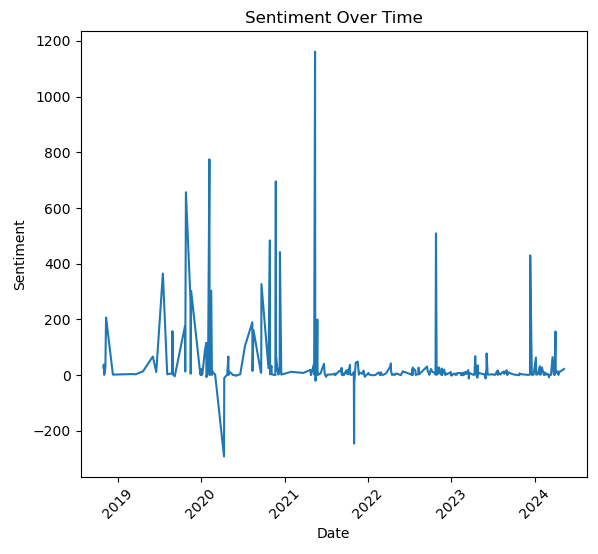
\includegraphics[width=\textwidth]{figures/line-chart.png}
    \end{subfigure}
    \begin{subfigure}{0.49\textwidth}
        \centering
        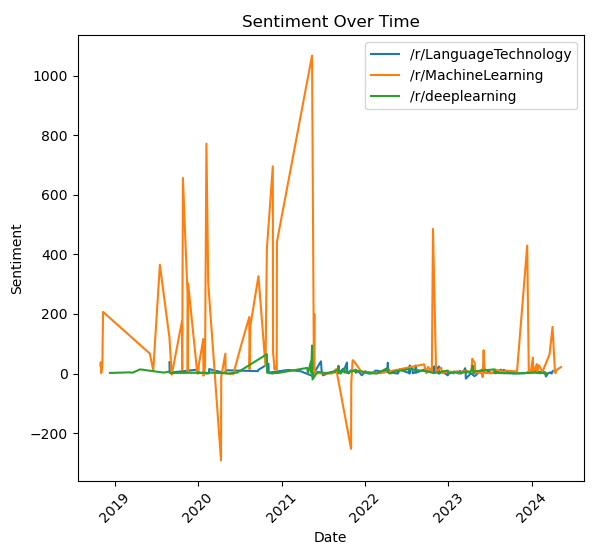
\includegraphics[width=\textwidth]{figures/split-line-chart.png}
    \end{subfigure}
    \caption{Example line charts with subreddit splitting enabled and disabled.}
\end{figure}

The pie chart represents the distribution of sentiment classifications within the dataset as a whole. Pie charts are great for showing the proportions of sentiment classes within the whole dataset, which makes them intuitive to the user, giving easy insight into which sentiment category dominates and how sentiment is distributed.

Finally, the bar chart compares the total sentiment scores across different subreddits. They are ideal for comparative analysis as they clearly display proportional quantities for different groups (in this case, subreddits),  allowing for clear visual indication of which subreddits and queries have the highest/lowest sentiment scores.

\begin{figure}[h]
    \centering
    \begin{subfigure}{0.49\textwidth}
        \centering
        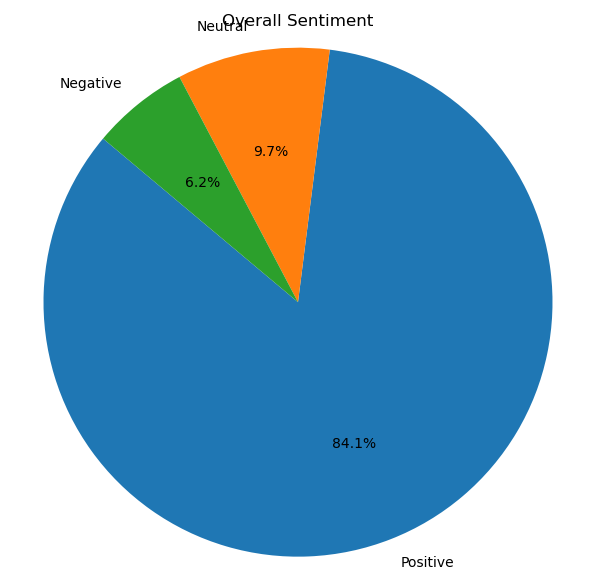
\includegraphics[width=\textwidth]{figures/pie-chart.png}
    \end{subfigure}
    \begin{subfigure}{0.49\textwidth}
        \centering
        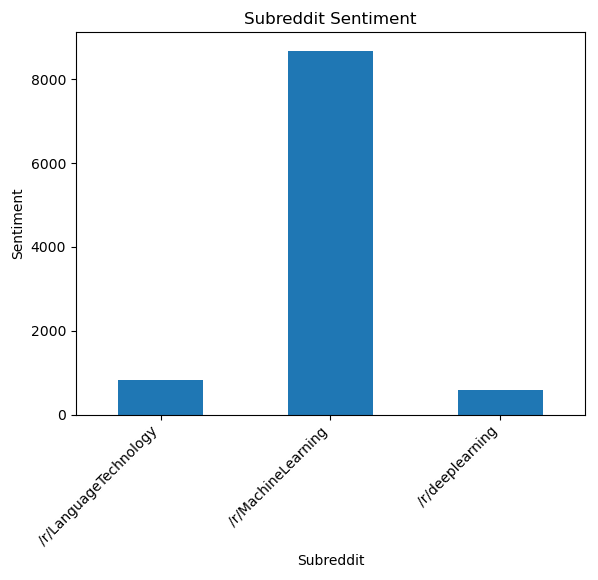
\includegraphics[width=\textwidth]{figures/bar-chart.png}
    \end{subfigure}
    \caption{Example pie and bar chart.}
\end{figure}

For further insight into the implementation of these charts, visit the GitHub repository \citep{sentimentanalysistool}.

\section{Graphical User Interface}

The GUI of the application (\pinline{toolkit/ui/interface.py}) serves as the means by which the user can interact with the functionality of the back-end processes. It is designed to provide an intuitive and user-friendly experience, while keeping performance and responsiveness to a high standard. This section outlines the architecture and components of the GUI, highlighting the core aspects such as the distinct windows and the use of parallel programming for long-running tasks. For the purpose of this application, the \pinline{QtPy} library was used, as it excels at creating complex, responsive, and user-friendly interfaces, as well as providing parallelism features.

    \subsection{Main Window}
    The \pinline{MainWindow} class, inheriting from \pinline{QtPy}'s \pinline{QMainWindow}, creates the main application, it displays widgets that link to the core functionalities of the program in an accessible format. The layout is built up by embedding other layouts and widgets within each other, creating an interface which is complex but pleasant to use. 

    \begin{figure}[h]
    \centering
        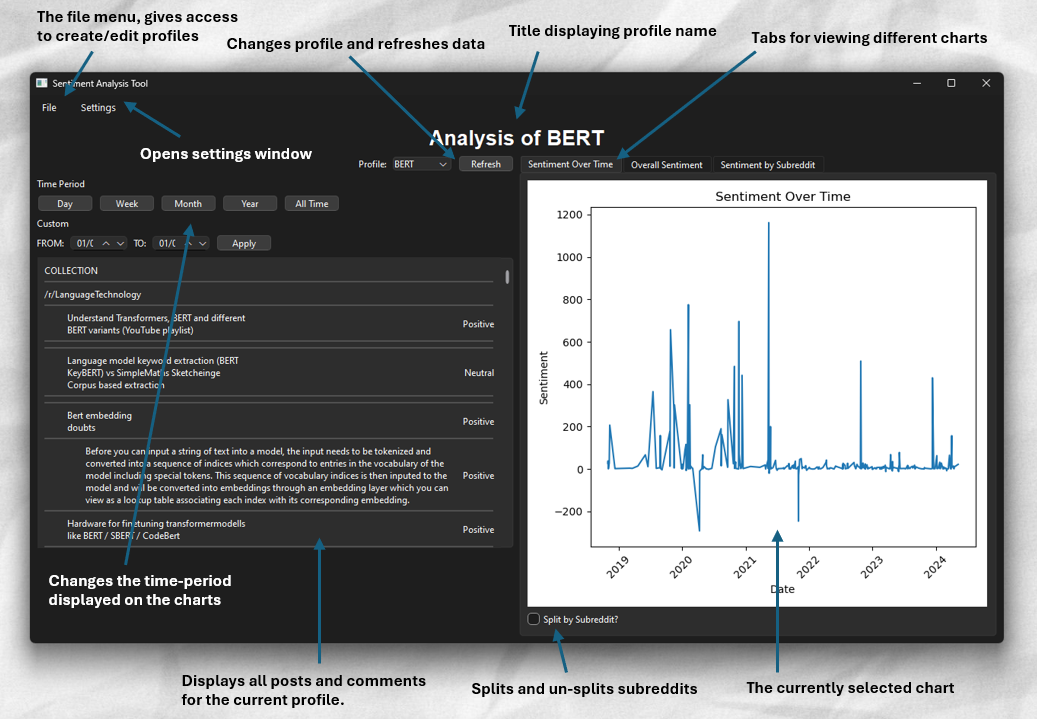
\includegraphics[width=0.95\textwidth]{figures/main-window-labels.png}
    \caption{The main window of the application.}
    \end{figure}

    As can be seen in the provided figure, the window consists of several main elements: a menu bar, a profile changer, a time period editor, a scrollable widget featuring all posts for the profile, and an area with tabs displaying different charts. Each distinct area is built up using layouts and widgets embedded in parent layouts, which are used as building blocks for the GUI. For example, the time period editor is built up through several different \pinline{MainWindow} methods, namely: 

    \begin{itemize}
        \item \pinline{self._make_time_period_layout()}
        \item \pinline{self._make_custom_time_layout()}
        \item \pinline{self._make_time_changer_layout()}
    \end{itemize}

    The time period layout consists of five buttons to change the time period to either the last twenty-four hours, week, month, year, or all-time.

    The \pinline{QtPy} object \pinline{QHBoxLayout} is used to create a layout consisting of a row of horizontal `boxes', which are used for placing widgets (or other layouts) into. Due to the one-dimensional layout of this, it is necessary to embed layouts \pinline{QHBoxLayout} and \pinline{QVBoxLayout} within each other to achieve a complex GUI. Once the layout is created, a \pinline{QPushButton} widget is created, connected to the \pinline{self._time_period_day()} function, and added to the layout as such (code reduced for simplicity):

    \begin{python}
def _make_time_period_layout(self):
    layout = QHBoxLayout()
    button_day = QPushButton("Day")
    button_day.clicked.connect(self._time_period_day)
    layout.addWidget(button_day)
    layout.addStretch()
    return layout
    \end{python}

    Following this, another layout is created to enable the user to select a more specific time period using selection boxes. This layout is implemented in a similar way, however, to prevent the charts updating every time the user increments or decrements the start/end date, a button labelled `Apply' is also added. For this button to work and pass the new start/end date to its connected function, a lambda function must be created as the passed function.

    \begin{python}
def _make_custom_time_layout(self):
    layout = QHBoxLayout()
    selector_from = QDateEdit()
    selector_to = QDateEdit()
    apply = QPushButton("Apply")
    apply.clicked.connect(lambda: self._set_dates(selector_from, selector_to))
    # Add widgets and return layout
    \end{python}

    These are then added to their parent layout, itself being a child of other layouts.

    \begin{python}
def _make_time_changer_layout(self):
    layout = QVBoxLayout()
    time_period_layout = self._make_time_period_layout() 
    custom_time_layout = self._make_custom_time_layout() 
    layout.addLayout(time_period_layout)
    layout.addLayout(custom_time_layout)
def _make_left_layout(self):
    layout.addLayout(self._make_time_changer_layout())
def _make_main_layout(self):
    layout.addLayout(self._make_left_layout())
    \end{python}

    Finally, the finished layout, made up of dozens of child layouts and widgets, is set as the layout of the window itself in \pinline{MainWindow.__init__()}.

    \begin{python}
class MainWindow(QMainWindow):
    def __init__(self, *args, **kwargs):
        self.widget = QWidget(self)
        self.setCentralWidget(self.widget)
        self.layout = self._make_layout()
        self.widget.setLayout(self.layout)  
    \end{python}

    To see the \pinline{MainWindow} in full detail, see the GitHub \citep{sentimentanalysistool}.

    \subsection{Profile Editor}
    The \pinline{ProfileEditorWindow} is a dedicated interface for managing the brand profiles. It allows the user to create, edit, and delete profiles; each profile contains information about which subreddits to monitor and analyse, and which search terms, if any, to query.

    \begin{figure}[h]
        \centering
            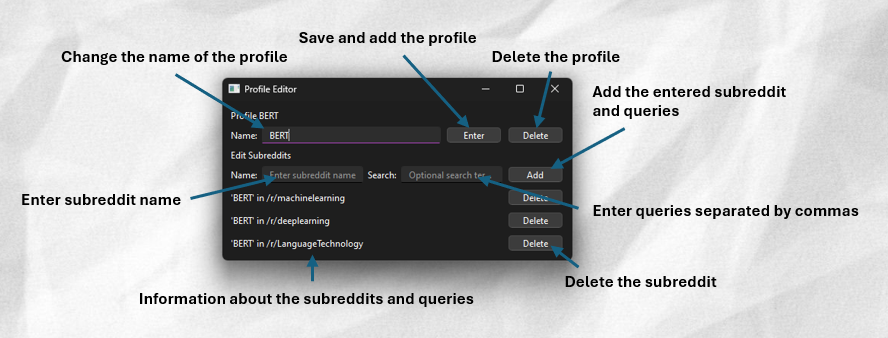
\includegraphics[width=0.95\textwidth]{figures/profile-editor-window-labels.png}
        \caption{The profile editor window.}
    \end{figure}

    In order for this window to communicate with the main window, a \pinline{pyqtSignal} object must be defined, which allows the transmission of signals between different objects in a program. This signal object is then used in the \pinline{ProfileEditorWindow._update()} function to \pinline{emit()} a signal that is picked up by the \pinline{MainWindow}. This allows the main window to update every time the profile editor window does.

    \begin{python}
class ProfileEditorWindow(QWidget):
    submit_clicked = pyqtSignal()
    def _update(self):
        self.submit_clicked.emit()

# Inside MainWindow
self.window_profile_editor.submit_clicked.connect(self._update)
    \end{python}

    To gain more insight into the workings of the \pinline{ProfileEditorWindow}, please refer to the GitHub repository \citep{sentimentanalysistool}.

    \subsection{Settings}
    The \pinline{SettingsWindow} class allows the user to customise various settings and preferences. It is divided into several distinct tabs for organisation and ease of use, such as General, Analysis, Personalisation, etc.

    \begin{figure}[h]
        \centering
            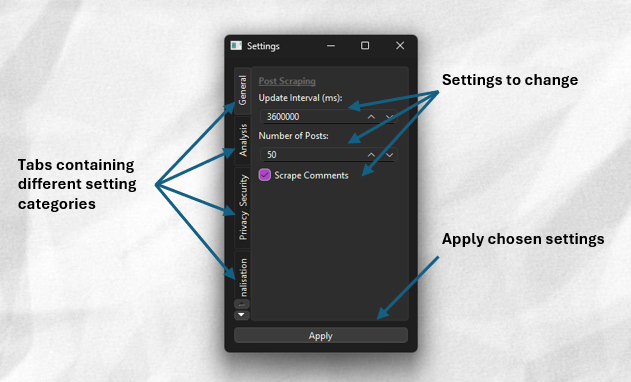
\includegraphics[width=0.95\textwidth]{figures/settings-window-labels.png}
        \caption{The settings window.}
    \end{figure}
    
    \begin{itemize}
        \item \textbf{General}: user can change the update interval, number of posts to scrape, and toggle comment scraping.
        \item \textbf{Analysis}: provides options for text processing such as lowercase, lemmatisation, and \pinline{BeautifulSoup} parsing, as well as model configurations like toggling cross-validation and changing the confidence threshold.
        \item \textbf{Privacy \& Security}: settings such as encryption can be toggled here (no functionality implemented).
        \item \textbf{Personalisation}: allows the user to customise the appearance of the application, such as font, colour, and chart styling (no functionality implemented).
        \item \textbf{Export \& Sharing}: allows the user to initiate a data export or share analyses (no functionality implemented).
        \item \textbf{Feedback \& Support}: provides the user with links to the creator's LinkedIn profile, send the creator an email, or visit the codebase on GitHub.
    \end{itemize}

    Each of these tabs have their own unique settings, for example, in the `General' tab, the update interval can be set using a \pinline{QSpinBox} that sets the interval in milliseconds, allowing a range anywhere from one second to twenty-four hours.

    \begin{python}
update_interval_spinbox = QSpinBox()
update_interval_spinbox.setMinimum(1000)
update_interval_spinbox.setMaximum(86400000)
update_interval_spinbox.setValue(toolkit.get_config("update_interval"))
update_interval_spinbox.valueChanged.connect(lambda value, name="update_interval": self._update_setting(name, value))
    \end{python}

    To prevent constant updates to the \pinline{MainWindow}, all settings changes are deferred inside of the \pinline{self.settings} dictionary until the user clicks the `Apply' button.

    \begin{python}
def _update_setting(self, name, value):
    self.settings[name] = value
    \end{python}

    This window uses similar functionality as the \pinline{ProfileEditorWindow} to communicate with the \pinline{MainWindow} using a \pinline{pyqtSignal} object, which this time is sent when the user clicks `Apply' and \pinline{self._apply_settings()} is called.

    \begin{python}
class SettingsWindow(QWidget):
    submit_clicked = pyqtSignal()
    def _apply_settings(self):
        for setting_name, value in self.settings.items():
            toolkit.set_config(setting_name, value)
        self.submit_clicked.emit()
    \end{python}

    \subsection{Parallelism for Long-Running Tasks}
    To ensure the application runs smoothly and efficiently, specifically during resource-intensive tasks such as social media scraping and analysis, \pinline{QtPy}'s parallelism features are used. Running tasks in parallel allows the application to perform multiple tasks simultaneously, significantly reducing the time required to execute. It is also ensures that the GUI stays responsive during these tasks rather than freezing, meaning the user can continue to interact with and use the program unimpeded.

    In the \pinline{MainWindow}, parallelism is employed in the execution of two functions: \pinline{self._collect_new_posts()} and \pinline{self._train_model()}, both of which are long-running tasks which would freeze the application for an undesirably extended period of time without parallelism. Initially, the class defines a \pinline{self.threadpool} storing a \pinline{QtPy.QThreadPool} object, which handles the queuing and execution of `workers'.

    \begin{python}
class MainWindow(QMainWindow):
    def __init__(self, *args, **kwargs):
        self.threadpool = QThreadPool()
    \end{python}

    To be able to use the \pinline{QThreadPool}, a new class \pinline{Worker} is defined, inheriting from \pinline{QtPy.QRunnable}, with the function to execute passed as an argument to it's \pinline{run()} method, using the \pinline{@pyqtSlot()} decorator.

    \begin{python}
class Worker(QRunnable):
    def __init__(self, fn: callable, *args, **kwargs) -> None:
        super(Worker, self).__init__()
        self.fn = fn
        self.signals = WorkerSignals()
    @pyqtSlot()
    def run(self):
        try:
            result = self.fn(*self.args, **self.kwargs) # Execute the passed function
        except: # Emit exception
        else:
            self.signals.result.emit(result)
        finally:
            self.signals.finished.emit()
    \end{python}

    Finally, the two long-running functions are called using multithreading by passing them as a callable upon a \pinline{Worker} creation. The program starts the worker and waits for the `finished' signal from to be emitted, so that it can call \pinline{self._update()}.

    \begin{python}
def _collect_new_posts(self):
    worker = Worker(lambda: self.collector.scrape_posts(toolkit.get_config('n_posts')))
    worker.signals.finished.connect(self._update)
    self.threadpool.start(worker)

def _train_model(self):
    worker = Worker(self.model.train)
    worker.signals.finished.connect(self._update)
    self.threadpool.start(worker)
    \end{python}